\documentclass{scrartcl}

\usepackage[utf8]{inputenc}
\usepackage[english]{babel}
\usepackage{amsmath, amssymb, amsthm}
\usepackage{fancyhdr}
\usepackage{esvect}
\usepackage{tikz}
\usetikzlibrary{angles,quotes}
\usepackage{xcolor}
\usepackage{pdfpages}
\usepackage{graphicx}
\usepackage{listings}
\usepackage{siunitx}
% \usepackage{pgfplots}
\usepackage{nowidow} % Hurenkinder und Schusterjungen verhindern
\clubpenalty10000
\widowpenalty10000
%\displaywidowpenalty10000
\emergencystretch 1.5em
\setlength{\parindent}{0em}
% Links in references
\usepackage{hyperref}
% Image positioning
\usepackage{float}

\pagestyle{fancy}

\definecolor{codegreen}{rgb}{0,0.6,0}
\definecolor{codegray}{rgb}{0.5,0.5,0.5}
\definecolor{codepurple}{rgb}{0.58,0,0.82}
\definecolor{backcolour}{rgb}{0.95,0.95,0.92}
\lstdefinestyle{mystyle}{
    backgroundcolor=\color{backcolour},   
    commentstyle=\color{codegreen},
    keywordstyle=\color{magenta},
    numberstyle=\tiny\color{codegray},
    stringstyle=\color{codepurple},
    basicstyle=\ttfamily\footnotesize,
    breakatwhitespace=false,         
    breaklines=true,                 
    captionpos=b,                    
    keepspaces=true,                 
    numbers=left,                    
    numbersep=5pt,                  
    showspaces=false,                
    showstringspaces=false,
    showtabs=false,                  
    tabsize=2
}
\lstset{style=mystyle}

\begin{document}

\rhead{}
\lhead{Janik Schmid (xxxxxxx), Lutz Bader (xxxxxxx), Felix Hausberger (3661293)}

% set counter 1 lower than the exercise number to have a correct section counter
\setcounter{section}{0}

\section{Algorithms and Data Structures 2 - Exercises 1}

\section{Problem 1}

\begin{enumerate}
    \item \textbf{Give the important differences between a normal priority queue and an addressable priority queue.}
    
    Normal priority queues maintain a set $M$ of Elements with Keys under the following operations: \\
    $M.build(\{e_1,...,e_n\}): M :=\{e_1,...,e_n\}$ \\
    $M.insert(e): M := M \cup \{e\}$ \\
    $M.min: return \; min \; M$ \\
    $M.deleteMin: e:=min \; M; M :=M \ \{e\}; return \; e$

    Addressable priority queues additionally support operations on arbitrary elements addressed by an element handle $h$: \\
    $insert$: As before but return a handle to the element inserted. \\
    $remove(h)$: Remove the element specified by handle $h$. \\
    $decreaseKey(h,k)$: Decrease the key of the element specified by handle $h$ to $k$. \\
    $Q_1.merge(Q_2): Q_1:= Q_1 \cup Q_2; Q_2 := \emptyset$.

    \item \textbf{Compare the running time of a merge operation for pairing heaps and binary heaps.}
    
    Pairing Heap: merge $O(1)$ \\
    The minPtr is updated and an addressable priority queue is simply attached to the forest.
    
    Binary Heap: merge
    
    

\end{enumerate}


\subsection{Problem 2}

\begin{enumerate}
    \item \textbf{Prove the general lower bound for addressable priority queues of $\Omega$(log n) for deleteMin under
the condition that insert runs in constant time.}

\item \textbf{Why does this bound not have to hold if insert is allowed to consume more time?}

\end{enumerate}


\subsection{Problem 3 (4 points)}

\textbf{For a very big festival, you are responsible for the bar. For this task, you designed a bar robot (aka Bender) that mixes excellent cocktails. The ingredients are stored in big boxes. But exactly here is the problem: you have to make sure that none of the boxes runs empty. On the other hand, you also want to enjoy the evening and not constantly check all of the boxes. To deal with this problem, there is only one solution: a refill display! Unfortunately, the only displays available are the ones that can display one line only.}

\textbf{It is clear that this line should display the most urgently need ingredient. The goal is to design an algorithm that keeps the display up to date.}

\begin{enumerate}
    \item \textbf{As a base for you algorithm, think about a data structure to efficiently implement your algorithm. Assume that the number of ingredients for a specific cocktail is significantly smaller than the number of ingredients totally available.}
    
    To model the refill display, that can only show the most urgent ingredient, an addressable priority queue will be used. An addressable one is needed, as the ingredients decrease in each box throughout the evening, which can be modeled only with the \textit{decreaseKey(h: Handlke, k: Key)} function of addressable priority queues. The priority is represented by how much each box is filled. The one that is filled the least will be shown on the display, it is the \textit{minimum} element in the priority queue. With \textit{deleteMin()} an empty box can be removed and a new box can be added by \textit{insert(e)}. The \textit{remove(h: Handle)} function is not needed as one can anyways only look at one box at most by the restrictions of the display (the one that is filled the least by using \textit{min()}). As the number of ingredients for a specific cocktail is significantly smaller than the number of ingredients totally available, a lot of cache misses might occur in the application. To counter this a \textit{Binary Heap} implementation will be chosen that reduces the amount of cache misses in practice as it uses addressable arrays/vectors internally instead of pointers like a \textit{Pairing Heap} or \textit{Fibonacci Heap} implementation. Thus this leads to better performance in practice even if the \textit{decreaseKey(h: Handlke, k: Key)}, \textit{deleteMin()} and \textit{insert(e)} function only run in \textit{O(log n)} in theory. On implementation level, a vector-like data structure will be used that is organized by an implicit tree representation maintaining the heap property/invariant.

	\item \textbf{Design a function MixDrink( recipe ), that operates on your data structure. Give Pseudocode. Your data structure has to be updated! Other functions of the robot don’t have to be “programmed”.}
	
	\begin{lstlisting}[caption=The function MixDrink( recipe )]
		public Cocktail MixDrink( recipe ) {
			Cocktail cocktail = new Cocktail();
			for ingredient in recipe {
				unsigned int amount = ingredient.amount;
				IngredientBox box = this.fetchIngredientBox(ingredient.name);
				if(box.fill >= amount) {
					cocktail.add(box.remove(amount));
					# decreaseKey calls siftUp() internally
					displayPQ.decreaseKey(ingredient.name, box.fill);
				} else {
					amount -= box.fill
					cocktail.add(box.remove(box.fill));
					displayPQ.decreaseKey(ingredient.name, 0);
					
					this.throwToTrash(box);
					box = this.getNewIngredientBox(ingredient.name);
					# deleteMin calls siftDown() internally
					displayPQ.deleteMin();
					# insert calls siftUp() internally
					displayPQ.insert(ingredient.name, box.fill);
					
					cocktail.add(box.remove(amount));
					displayPQ.decreaseKey(ingredient.name, box.fill);
				}
			}
			return cocktail;
		}
	\end{lstlisting}

	\item \textbf{When a box is exchanged, your data structure has to be updated as well. Describe what consequences the exchange has on your data structure.}
	
	There are actually two possibilities. Either one calls \textit{deleteMin()} and \textit{insert(e)} right afterwards which leads to recursive \textit{siftDown()} and \textit{siftUp()} operations or one supports an \textit{increaseKey(h: Handle, k: Key)} function, that leads to only one recursive \textit{siftDown()} call. Nevertheless, \textit{O(log n)} swaps need to be performed. 
	
\end{enumerate}

\subsection{Problem 4}

\textbf{The definition of a pairing heap does not state which elements are neighbors. For the solution of the next tasks we assume a sorted list of roots (by insertion order) and neighborhood induced by this. Given is a Pairing Heap in the following state.}

\begin{enumerate}
    \item \textbf{Give a very short sequence of operations that creates this state.}
    
    insert(0) \\
    insert(1) \\
    insert(2) \\
    insert(3) \\
    insert(4) \\
    insert(5) \\
    insert(6) \\
    deleteMin() \\
    insert(0) \\
    deleteMin() \\
    insert(0) \\
    deleteMin() \\
    insert(8) 
    
    \item \textbf{Execute the following operations step by step on the given heap and draw the intermediate state of the heap after each operation: deleteMin(), insert(9), decreaseKey(a,1), remove(b).}

    \begin{center}
        \makebox[\textwidth]{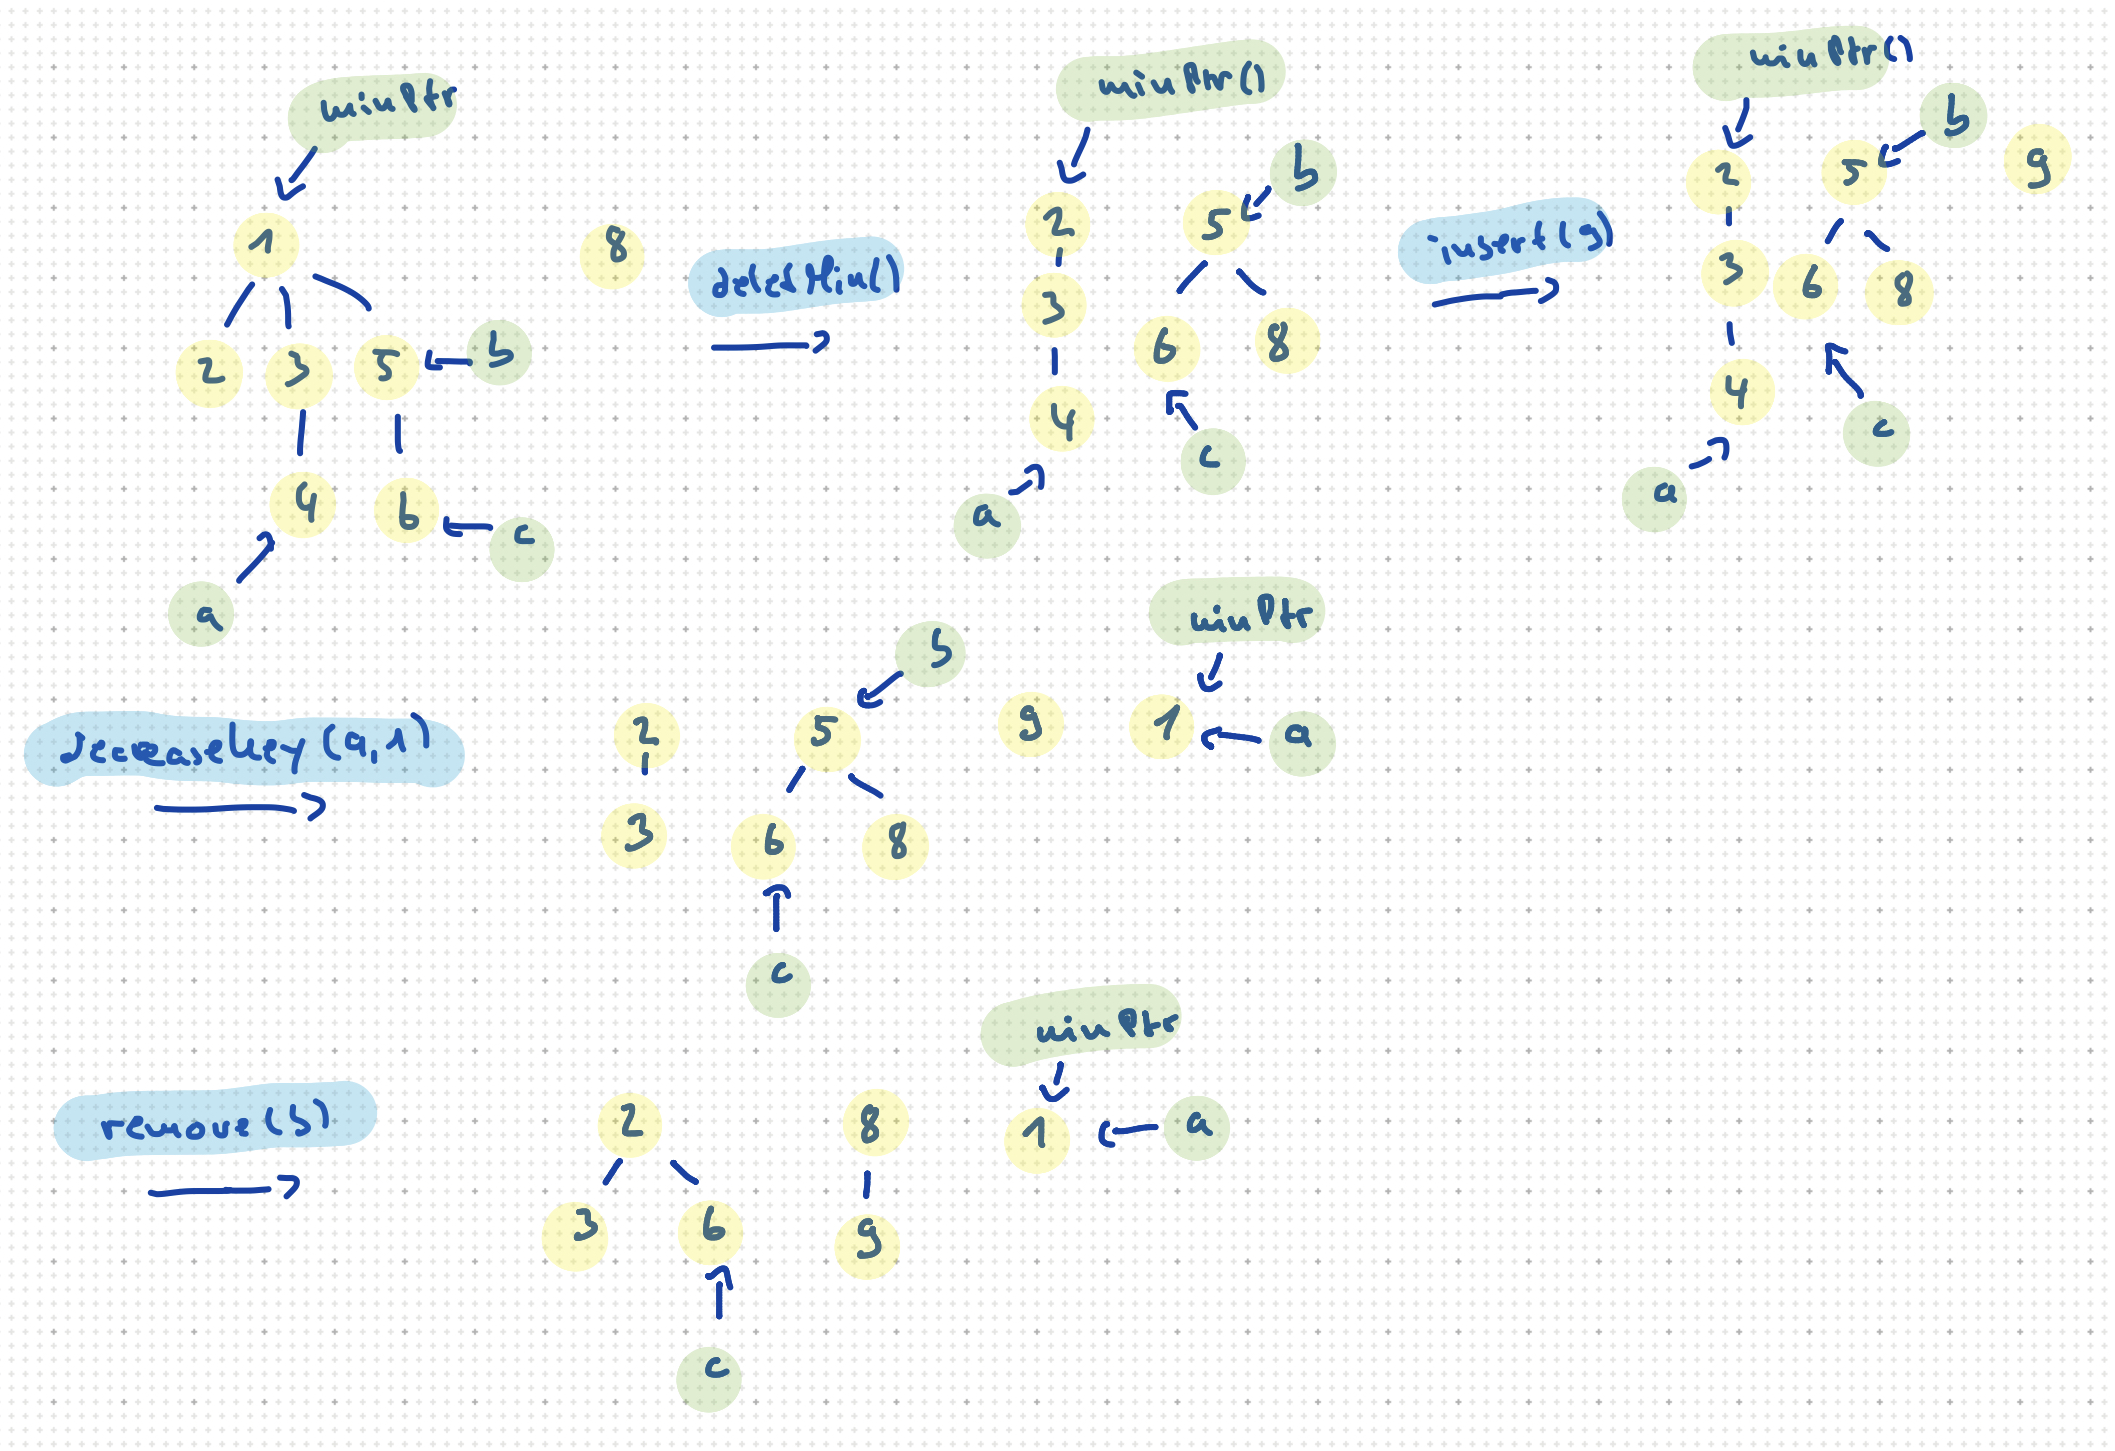
\includegraphics[width=\textwidth]{images/exercise_4.jpeg}}
    \end{center}

\end{enumerate}

\end{document}
